\documentclass[conference]{IEEEtran}
\IEEEoverridecommandlockouts
% The preceding line is only needed to identify funding in the first footnote. If that is unneeded, please comment it out.
\usepackage{cite}
\usepackage{amsmath,amssymb,amsfonts}
\usepackage{algorithmic}
\usepackage{graphicx}
\usepackage{textcomp}
\usepackage{xcolor}
\usepackage{url}
\usepackage[colorlinks]{hyperref}
\usepackage{listings}
\usepackage{tikz}
\usepackage{tkz-euclide}
\usepackage{svg}
\usepackage{pdfpages}

\usetikzlibrary{shapes,positioning,shapes.gates.logic}

\tikzset{ell/.style={circle,draw,minimum height=0.2cm,minimum width=0.2cm,inner sep=0.15cm}}
\tikzset{rec/.style={rectangle,draw,minimum height=0.5cm,minimum width=0.5cm,inner sep=0.2cm}}
\tikzset{trp/.style={trapezium,draw,trapezium left angle=120, trapezium right angle=120, minimum height=0.5cm}}


%New colors defined below
\definecolor{codegreen}{rgb}{0,0.6,0}
\definecolor{codegray}{rgb}{0.5,0.5,0.5}
\definecolor{codepurple}{rgb}{0.58,0,0.82}
\definecolor{backcolour}{rgb}{0.95,0.95,0.92}

%Code listing style named "mystyle"
\lstdefinestyle{mystyle}{
  backgroundcolor=\color{backcolour}, commentstyle=\color{codegreen},
  keywordstyle=\color{magenta},
  numberstyle=\tiny\color{codegray},
  stringstyle=\color{codepurple},
  basicstyle=\ttfamily\footnotesize,
  breakatwhitespace=false,         
  breaklines=true,                 
  captionpos=b,                    
  keepspaces=true,                 
  numbers=left,                    
  numbersep=5pt,                  
  showspaces=false,                
  showstringspaces=false,
  showtabs=false,                  
  tabsize=2
}

%"mystyle" code listing set
\lstset{style=mystyle}


\def\BibTeX{{\rm B\kern-.05em{\sc i\kern-.025em b}\kern-.08em
    T\kern-.1667em\lower.7ex\hbox{E}\kern-.125emX}}
\begin{document}

\title{Improving GPT Penetration Testing Using Prompt Engineering Techniques and Newly Released Features
\thanks{}
}
\author{\IEEEauthorblockN{Daniel Lichtenberger}
\IEEEauthorblockA{\textit{Department of EECS} \\
\textit{Texas A\&M University-Kingsville}\\
Kingsville, USA \\
daniel.lichtenberger@students.tamuk.edu
}
\and
\IEEEauthorblockN{Mengxiang Jiang}
\IEEEauthorblockA{\textit{Department of EECS} \\
\textit{Texas A\&M University-Kingsville}\\
Kingsville, USA \\
mengxiang.jiang@students.tamuk.edu}
}

\maketitle

\begin{abstract}
    With the introduction of GPT-4 in early 2023, many researchers discovered capabilities of large language models (LLM) that were in the past lacking. One of these capabilities is penetration testing in the field of cybersecurity, which is the controlled hacking of a test server in order to discover and mitigate vulnerabilities. This allows security experts to automate some of the process since many of the tasks required are fairly routine. A framework for doing this called PentestGPT which was able to perform at the top 1\% of users at the penetration test website HackTheBox by using prompt engineering techniques. Prompt engineering is the modification of the input (prompt) in order to change the behavior of large language models to meet the needs of a specific task. In this paper we use some general purpose prompt engineering techniques as well as some newly released features of ChatGPT such as input image and web search to improve penetration testing results. Our results show that the general prompt engineering techniques were not very effective, but the newly released features were.
\end{abstract}

\section{Introduction} \label{sec:intro}
ChatGPT is a large language model (LLM) that generates automated responses that correlates with a response asked by users\cite{engman2023evaluation}. ChatGPT itself exploded in popularity that sparked greater curiosity in the field of artificial intelligence. The model itself has accumulated an information dataset that has expanded in more recent iterations with GPT-4 \cite{hariri2023unlocking}. Apart from ChatGPT, LLMs are becoming an investment that could affect the lives of people depending on their use and accessibility. Cybersecurity is one field that is currently being explored with LLMs such as ChatGPT. Penetration testing is one such topic in the realm of cybersecurity that is being tested with ChatGPT and the results that the model produces.

Penetration testing (pentest) started as a need to combat cybercrime from a dynamically involved cybersecurity environment by proactively trying to hack one's own machines\cite{deng2023pentestgpt}. From 2021, the FBI reported that data breaches caused monetary damages up to \$6.9 billion dollars\cite{heim2023convergence}.  Pentesting is becoming more of a demand as companies desire to have protection in case of an emergency. The process is very intensive and requires a dedicated security team to carry out methodical processes to complete\cite{applebaum2017analysis}. There are different levels of penetration testing known as white-box, black-box, and gray-box determined by the amount of knowledge from the system in question\cite{deng2023pentestgpt}.

Lately, there has been significant advancement in LLMs, demonstrating refined and nuanced comprehension of human-like text and proficiently completing a variety of tasks in multiple fields\cite{zhao2023survey}\cite{liu2023summary}. An interesting characteristic of LLMs is their emergent capabilities—capabilities not directly coded but developed during training\cite{wei2022emergent}. This enables them to undertake sophisticated tasks like reasoning, summarizing, answering questions, and solving domain-specific problems without the need for task-specific training. These capabilities highlight the transformative possibilities of LLMs in several sectors, cybersecurity and penetration testing in particular.

A mixture that both utilizes AI and penetration testing is a framework called PentestGPT\cite{heim2023convergence}. PentestGPT demonstrates pentesting capabilities by inputting generated responses from ChatGPT into making an automated penetration tester \cite{deng2023pentestgpt}. The framework uses 3 modules independent from one another to keep information on track due to the token limitations of ChatGPT. Each module serves a purpose in conducting responses suitable to their role on a penetration testing team. The modules follow a step-by-step process in order to successfully output a suitable response. The reasoning module passes its results to the generation module, and ends with the parsing module getting information from the generation module. PentestGPT showed promising results for 4 out of the 10 targeted HackTheBox\cite{hackthebox} machines at a cost of 131.5 US dollars, which is in the top 1\% of users on the site. It utilizes a technique called prompt engineering, the subject of the next paragraph\cite{white2023prompt}. However, one major downside of this framework is that it utilizes the OpenAI API to access GPT-4 rather than through the official web interface. This makes accessing newly released features more difficult or impossible in certain cases, some of which can greatly benefit penetration testing.

Similar to human dialogues, LLM conversations can take multiple diverse directions. This variability has spawned a novel research field known as prompt engineering, which is the use of certain instructions, called \textit{prompts}, to tailor the LLM to a specific task. This field is concentrated on devising prompts that yield the most accurate and valuable responses, and it remains a burgeoning science. White et al. created a catalog of various general prompt engineering patterns in order to improve the results of these conversations\cite{white2023prompt}. We employed some of these patterns for the purpose of improving penetration testing.

OpenAI has also been steadily improving their ChatGPT service, with regular updates published on their website \cite{releasenotes}. These updates are crucial in ensuring that the model remains current with the latest technological advancements. Regular updates also involve refining the underlying algorithms for improved accuracy, responsiveness, and user interaction. Some of these new features are relevant to the task of penetration testing, and we will utilize them to improve penetration testing.

The results of our experimentation suggest that the general prompt engineering patterns does not greatly improve penetration testing while some of the new features of ChatGPT does. This finding will allow penetration testers to more efficiently carry out their tasks.

\section{Methodology} \label{sec:approach}
In this section, we will cover the various techniques we used to try to improve GPT-4's penetration test performance.

\subsection{Flipped Interaction Pattern} \label{ssec:flipped}
One of the first steps of a penetration test is intelligence gathering\cite{ptes}. During this stage, the primary goal is to collect as much information as possible about the target system without actively engaging with it. This information will be used in later stages of the penetration test to identify vulnerabilities and potential attack vectors. Rather than manually going through the list of activities prescribed by the Penetration Testing Execution Standard (PTES), having the LLM ask the tester for information is a more active way of achieving this step. The Flipped Interaction Pattern is having the LLM drive the conversation and automatically ask questions until it has sufficient information to.complete a task or proceed to the next step \cite{white2023prompt}. For our purposes, an example prompt to initialize this is: “I would like you to ask me questions to do the reconnaissance step of a penetration test following the Penetration Testing Execution Standard. When you have enough information, notify me in order to proceed to the next stage.”

\subsection{Persona Pattern} \label{ssec:persona}
Often, users prefer the output of LLMs to maintain a consistent perspective or stance. For instance, performing a penetration test with the LLM acting as a cybersecurity expert could be beneficial. The purpose of this approach is to assign a “persona” to the LLM, guiding it in determining the kind of responses to generate and the specifics to emphasize\cite{white2023prompt}. Pentest GPT already does this with initializing its core modules, with a prompt starting with “You're an excellent cybersecurity penetration tester assistant”\cite{deng2023pentestgpt}. We employ a similar persona pattern for our penetration tests.

\subsection{Image Input} \label{ssec:image}
OpenAI added voice and image capabilities to ChatGPT on September 25, 2023\cite{releasenotes}. The image input allows ChatGPT to view one or more images in one input in order to solve visual problems. As the saying goes that "an image is worth a thousand words", this feature allows much more efficient input certain forms of data for analysis. Furthermore, the ability to process complex visual information, like network diagrams or user interface anomalies, allows for a deeper inspection of potential security weaknesses that might be overlooked when relying solely on textual data. We used this feature mainly to share screenshots of webpages in order to aid our penetration testing.

\subsection{Browsing and Search} \label{ssec:browsing}
OpenAI added web browsing and search capabilities to ChatGPT on May 12, 2023\cite{releasenotes}. This allows ChatGPT to browse the internet for information it does not know. A successful penetration test often needs the gathering of data about specific vulnerabilities, exploits, or security configurations, which involving searching the internet to fetch up-to-date information, best practices, and potential solutions from various authoritative sources. This includes accessing recent security advisories, exploit databases, and forums where cybersecurity communities discuss emerging threats and defenses. ChatGPT's ability to do this automatically and synthesize information from multiple sources into coherent insights allows penetration testers to stay informed about the latest security trends and techniques, making their testing process more efficient and effective. 

\subsection{Equipment and Test Server}
For the local machine, we use Parrot OS virtual machines as recommended by HackTheBox. For the server that we run the penetration test on, we chose the Codify machine on HackTheBox. This was released on November 4, 2023, so it is very recent and the vulnerabilities of the services on the machine are similarly freshly discovered, meaning ChatGPT is unlikely to know about them from its training data. As such, it must creatively solve the challenge rather than simply regurgitate a memorized solution.

\section{Results}

\subsection{Disclaimer}
During the experiments, a large amount of the tasks suggested by ChatGPT to successfully conduct the penetration test were dead ends, regardless of what techniques were used. Oftentimes it was just a lucky ordering of which services were listed earlier that happened to be vulnerable that made the test shorter, and if the output were generated again, the ordering would be different. To make the comparisons of the different techniques more balanced, only outputs that lead to actual progress on the penetration tests are considered for the results. 
\begin{table}[htbp]
  \caption{Performance Results}
  \begin{center}
  \begin{tabular}{|c|c|c|c|}
  \hline
  \textbf{Technique} & \textbf{Control} & \textbf{Flipped Interaction} & \textbf{Persona} \\
  \hline
  \textbf{word count} & 6832 & 9941 & 6429 \\
  \hline
  \textbf{character count} & 44204 & 61805 & 43149 \\
  \hline
  \end{tabular}
  \label{table:results}
  \end{center}
\end{table}
\subsection{Control}
In order to have a baseline for the prompt engineering techniques to compare to, a control penetration test was performed. Despite not using any of the techniques of the catalog, it still performed quite well with 6832 words and 44204 characters total to complete the penetration test. For a detailed account of this experiment, see Appendix \ref{sec:control}.

\subsection{Flipped Interaction}
The performance of the flipped interaction is quite a bit worse than the control at 9941 words and 61805 characters to complete the penetration test. This is largely due to providing much greater context regarding why it is asking those questions rather than simply stating an instruction on what to do. It also often forgets about asking questions and needs frequent reminders. Despite this, when conducting the penetration test using this method, we learned more detailed information about the test machine than in the other experiments, despite the output being longer. For a detailed account of this experiment, see Appendix \ref{sec:flipped}.

\subsection{Persona}
The persona prompt was able to finish the penetration test using 6429 words and 43149 characters, slightly better than the baseline. However, this is largely due to specifically telling it to give brief instructions on what to do, and even then the output was not much shorter than the baseline. In many cases, the instructions it provided were somewhat incomplete, and we had to interpolate the missing parts in order to successfully perform the instruction. Therefore the user experience was the least pleasant of the experiments even though in terms of the length of output it performed the best. For a detailed account of this experiment, see Appendix \ref{sec:persona}.

\subsection{Image Input}
In the case of our penetration tests, the webpages were mostly text and therefore there was no major difference between using screenshots as input versus the source code. However, the ease of use and readability of inputting images rather than pages of code made the testing experience better. And since GPT-4 has a rate limit of 40 inputs every three hours while multiple images can be sent as one input, allowing the tester potentially reduce the amount of wait times for additionally input slots in order to complete a penetration test.

\subsection{Browsing and Search}
Through the use of this feature, ChatGPT is able to quickly evaluate the promise of certain vulnerabilities. To quote ChatGPT itself:  ``In practice, a significant part of penetration testing involves identifying vulnerabilities and then assessing whether they are practically and ethically exploitable.'' An example of an impractical vulnerability is shown in Fig. \ref{fig:impractical}. \begin{figure}[htbp]
  \centering
  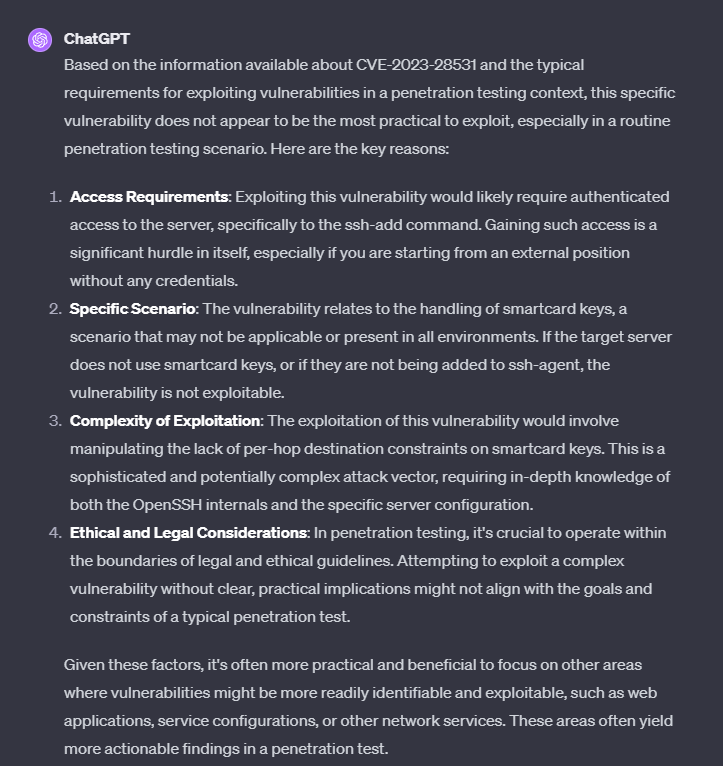
\includegraphics[width=\columnwidth]{search1.png}
  \caption{Impractical Vulnerability}
  \label{fig:impractical}
\end{figure} 
When a vulnerability is actually promising, ChatGPT often gives a link to to a proof of concept (PoC) of how to exploit this vulnerability and is willing to adapt it for specific purposes such as remote code execution (RCE). See Fig. \ref{fig:promising} for an example of a promising vulnerability.
\begin{figure}[htbp]
  \centering
  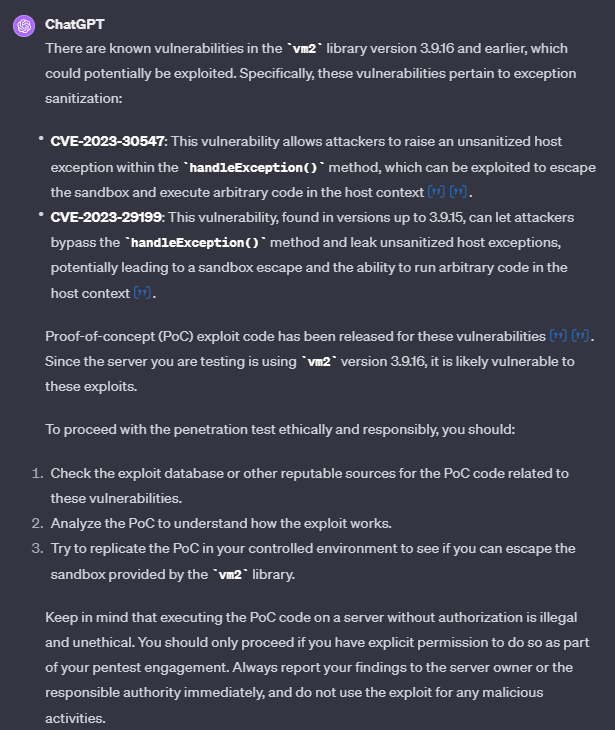
\includegraphics[width=\columnwidth]{search2.png}
  \caption{Promising Vulnerability}
  \label{fig:promising}
\end{figure}
This immediate access to relevant information eliminates the lengthy process of manual searching and analysis, allowing us to focus more on implementing attack strategies in order to complete the penetration test. As this part of penetration testing is often the most time intensive, even small improvements make a big difference.

\section{Conclusion}
The purpose of our experiments is to evaluate some general prompt engineering techniques as well as newly released features of ChatGPT on the performance of penetration testing. Our results indicate that the more general prompt engineering techniques are not especially effective and it is better to use more specific and elaborate prompt engineering techniques such as those of PentestGPT for better performance gains. However, the newly released features were effective in improving performance, especially the web browsing and searching feature. By properly utilizing this feature, penetration testers can save valuable time ignoring dead ends and instead focus on promising avenues to exploit.

\bibliographystyle{plain}
\bibliography{project}
\begin{appendices}
  \clearpage
  \section{Control} \label{sec:control}
  \clearpage
  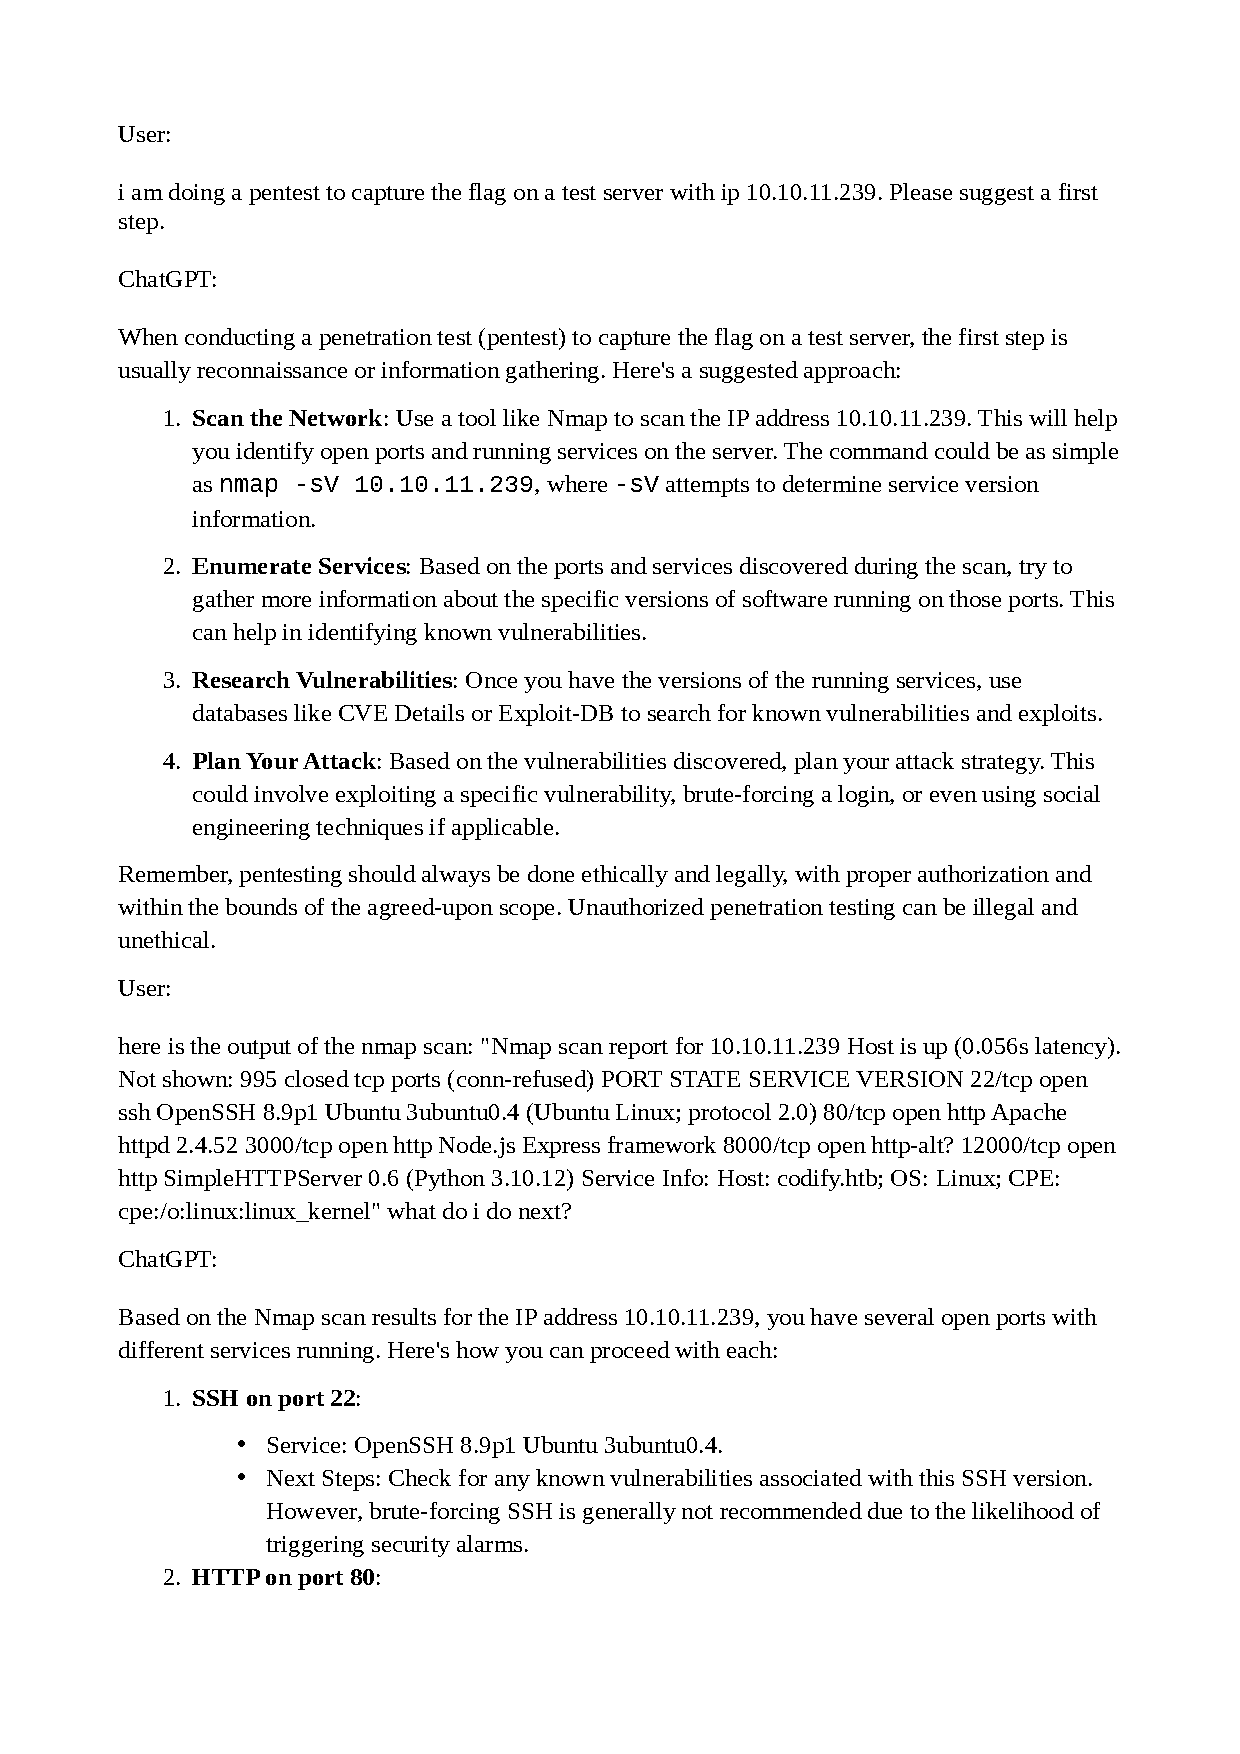
\includepdf[pages=-]{codify_control.pdf}
  \clearpage
  \section{Flipped Interaction} \label{sec:flipped}
  \clearpage
  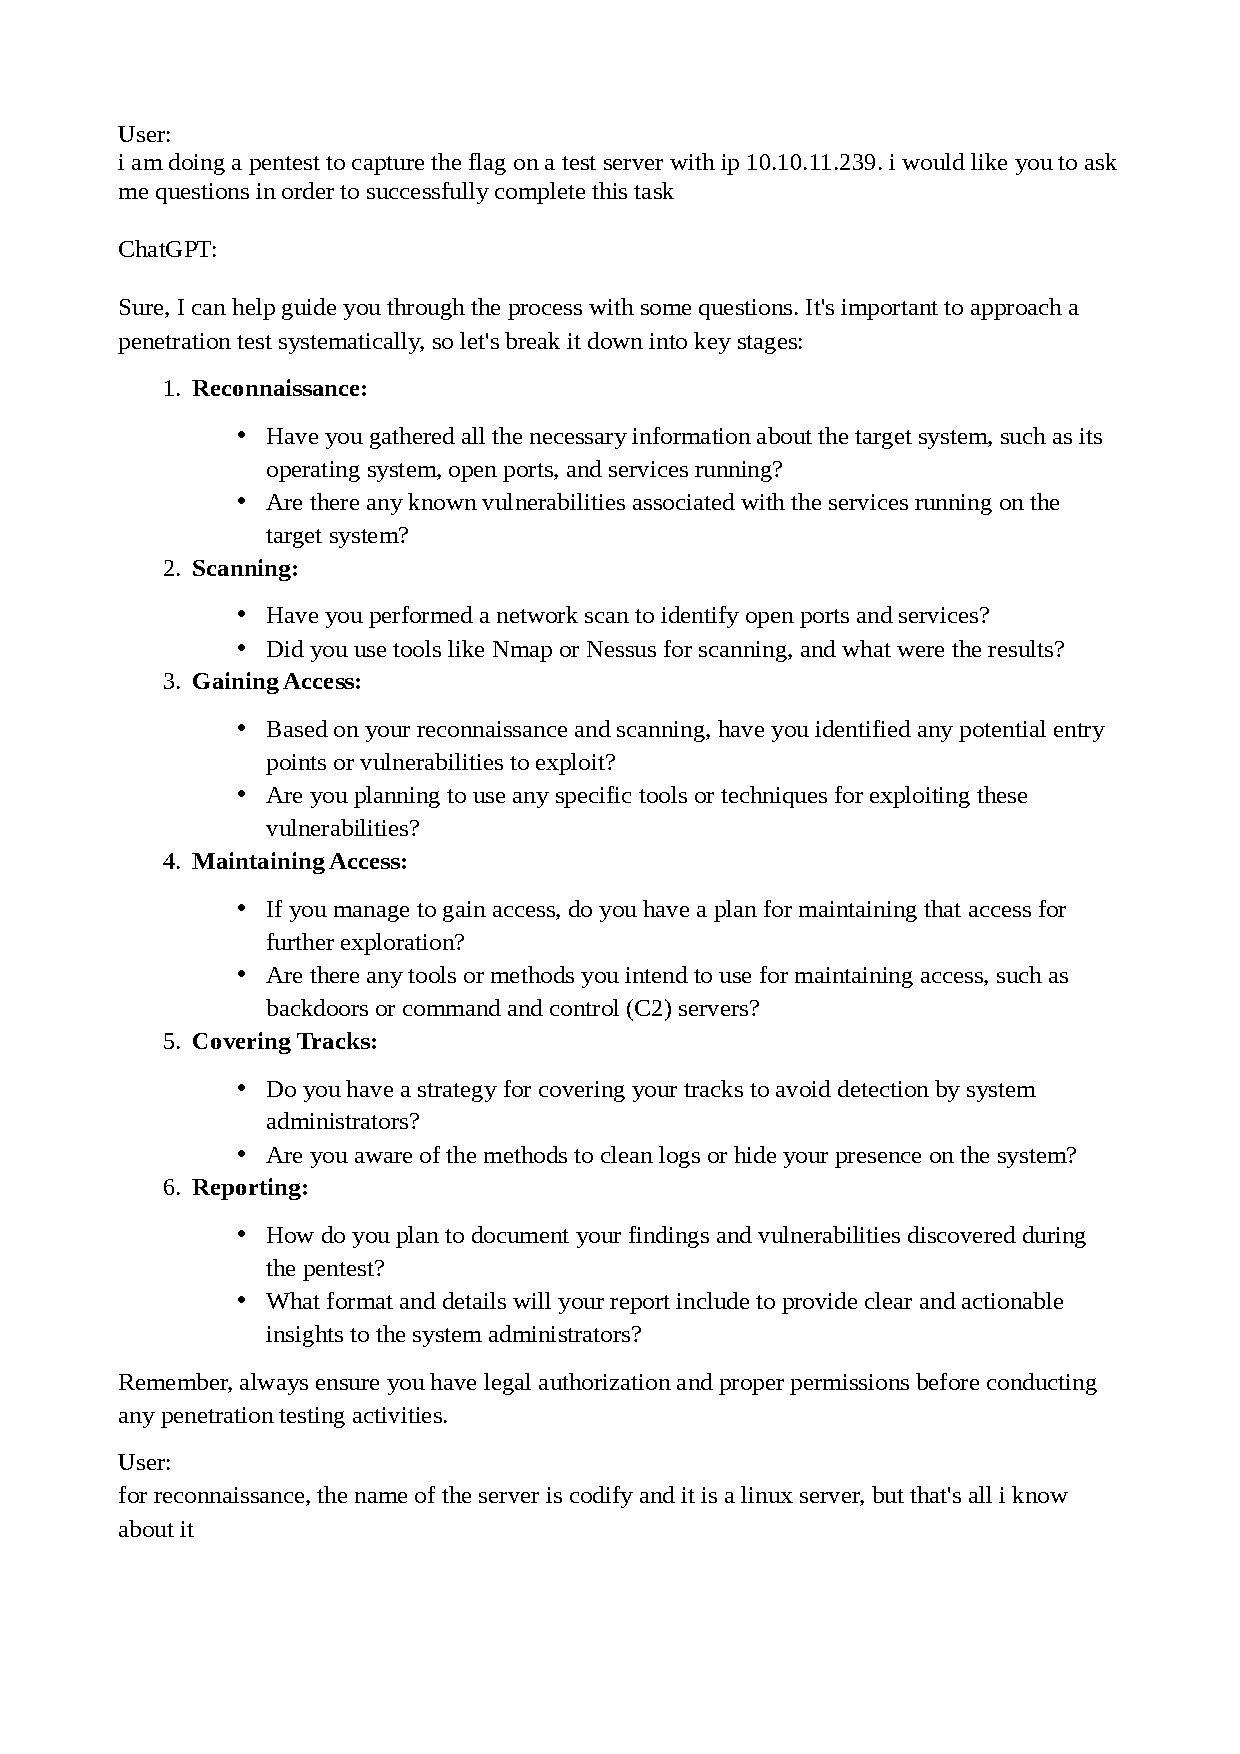
\includepdf[pages=-]{codify_flipped_interaction.pdf}
  \clearpage
  \section{Persona} \label{sec:persona}
  \clearpage
  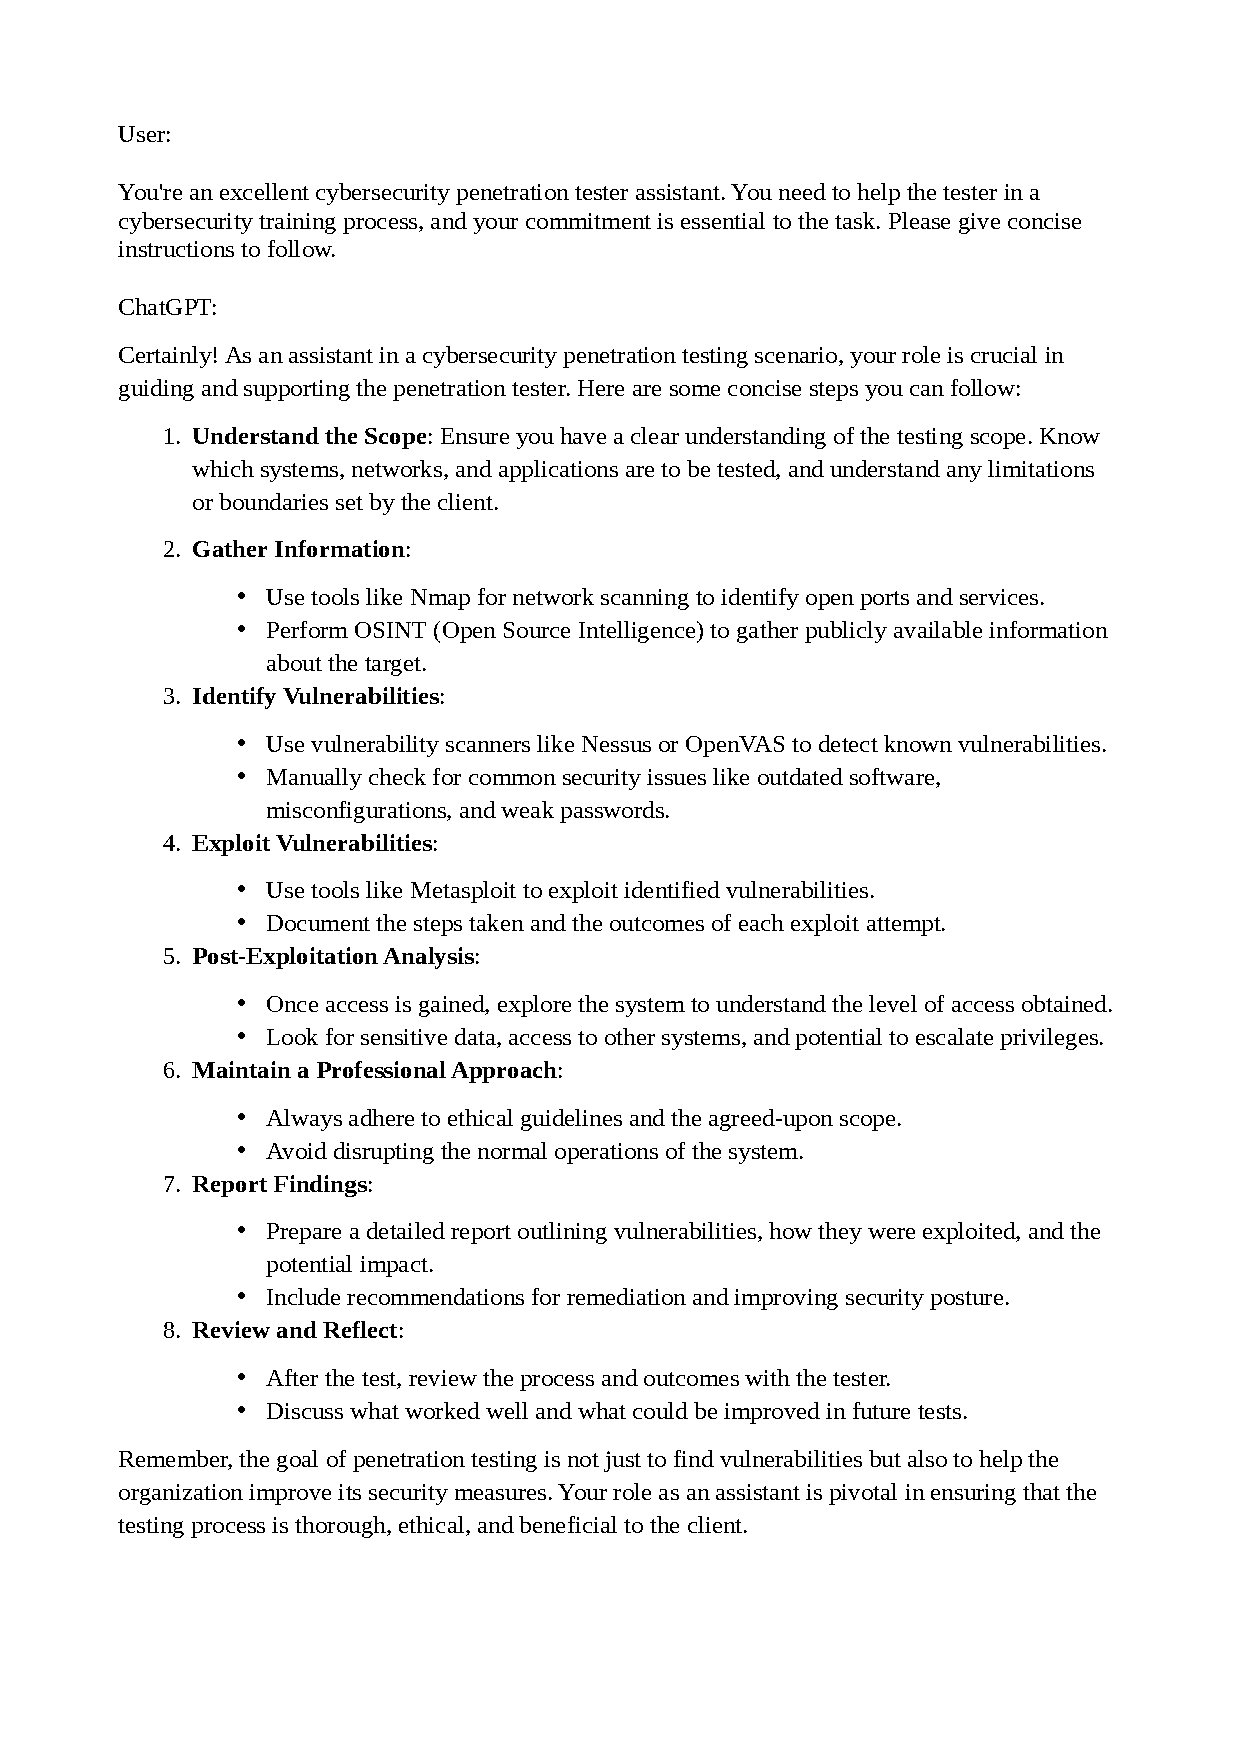
\includepdf[pages=-]{codify_persona.pdf}
\end{appendices}

\vspace{12pt}

\end{document}
